% This is samplepaper.tex, a sample chapter demonstrating the
% LLNCS macro package for Springer Computer Science proceedings;
% Version 2.20 of 2017/10/04
%
\documentclass[runningheads]{llncs}
%
\usepackage{graphicx}
% Used for displaying a sample figure. If possible, figure files should
% be included in EPS format.
%
% If you use the hyperref package, please uncomment the following line
% to display URLs in blue roman font according to Springer's eBook style:
% \renewcommand\UrlFont{\color{blue}\rmfamily}

\begin{document}
%
\title{Sports Object Recognition and Tracking\thanks{Supported by organization Leiden University.}}
%
%\titlerunning{Abbreviated paper title}
% If the paper title is too long for the running head, you can set
% an abbreviated paper title here
%
\author{Shreyansh Sharma\inst{1}\orcidID{S3772241} }
%
\authorrunning{S. Sharma et al.}
% First names are abbreviated in the running head.
% If there are more than two authors, 'et al.' is used.
%
\institute{Leiden University, Netherlands\\
\email{S3772241@vuw.leidenuniv.nl}}
%
\maketitle              % typeset the header of the contribution
%
\begin{abstract}
% The abstract should briefly summarize the contents of the paper in
% 15--250 words.
% TODO: Write abstract
% 
Sports object recognition and tracking is a challenging task in computer vision. 
This paper presents and compares different methods for object recognition and tracking in sports videos.
Th focus lies on utilizing pre-trained models to reduce the training time and improve the accuracy of the model.
Along with the comparison, a framework is proposed to evaluate the performance of the models.
The framework can be accessed at \url{https://github.com/shreyansh05s/SPORT}.
\keywords{DETR  \and DeepSort \and SportsMot.}
\end{abstract}
%
%
%
\section{Introduction}
% talk about dataset automatically generated and why it is important
% talk about the importance of object recognition and tracking in sports
% How this data can be used for downstream tasks
In recent years, the field of computer vision has seen a lot of progress in object recognition and tracking.
Improved object recognition and tracking can be used in many applications such as autonomous driving, surveillance, and sports analysis.
In sports, object recognition and tracking can be used to analyze the performance of the players and the team.
It can also be used to analyze the performance of the referee and the umpire.
The data generated from object recognition and tracking can be used for downstream tasks such as player tracking, player action recognition, and player pose estimation.

Object recognition and tracking in sports is a challenging task due to the fast movement of the players and the ball.
The players and the ball can be occluded by other players or the referee.
The players can also be occluded by the audience.
This makes it difficult to track the players and the ball.

In this paper, we present and compare different methods for object recognition and tracking in sports videos.
The focus lies on utilizing pre-trained models to reduce the training time and improve the accuracy of the model.
Along with the comparison, a framework is proposed to allow faster setup and evaluation of the models.

For the comparison, we use the SportsMot dataset \cite{cui2023sportsmot}.
The SportsMot dataset is a large-scale dataset for multi-object tracking in sports.
It contains videos of different sports such as basketball, football, and volleyball.
This makes it suitable for comparing different methods for object recognition and tracking in sports.
MOT-16 and MOT-17 datasets \cite{milan2016mot16} are also popular datasets for multi-object tracking.


\section{Related Work}
Usually, the task of object recognition and tracking is tackled in two steps.
First, the objects are detected in each frame of the video.
Second, the detected objects are tracked across the frames of the video.
This is also commonly known as the tracking-by-detection approach.
One such example for tracking-by-detection approach is the Deep SORT algorithm \cite{DBLP:journals/corr/abs-1907-03465}.

In recent years, there has also been a lot of progress in end-to-end object recognition and tracking.
But for the purpose of this paper, we will focus on the tracking-by-detection approach.

% One such example is the 


\subsection{Object Detection}
% Explain a little bit about how yolo made a breakthrough in object detection
% Then introduce DETR
% Explain how DETR works

Yolo \cite{yolo2015} made a breakthrough in object detection by introducing a single neural network for object detection.
Before Yolo, object detection was done using two neural networks.
The first neural network was used to generate the region proposals.
The second neural network was used to classify the region proposals.
This made the object detection pipeline slow and inefficient.

After Yolo, many other single neural network object detection models were introduced.
One such example is the DETR model \cite{detr2020}.
The DETR model uses a transformer \cite{transformer2017} to detect the objects in each frame of the video.
The transformer is a neural network architecture that uses attention to process the input data.
The DETR model uses a pre-trained ResNet-50 \cite{resnet2015} as the backbone.
The ResNet-50 is used to extract the features from the input image.
The extracted features are then passed to the transformer.
The transformer is used to detect the objects in the image.
The transformer outputs the bounding boxes and the class labels of the detected objects.


\subsection{Object Tracking}
The Deep SORT algorithm uses a pre-trained object detection model to detect the objects in each frame of the video.
The detected objects are then tracked across the frames of the video using the Kalman filter \cite{kalman1960new}.
The Kalman filter is used to predict the position of the objects in the next frame of the video.
The objects are then assigned to the predicted position based on the similarity between the predicted position and the detected position.
The similarity is calculated using the Hungarian algorithm \cite{hungarian1955}.
This process is repeated for each frame of the video.


\paragraph{Sample Heading (Fourth Level)}
The contribution should contain no more than four levels of
headings. Table~\ref{tab1} gives a summary of all heading levels.

\begin{table}
\caption{Table captions should be placed above the
tables.}\label{tab1}
\begin{tabular}{|l|l|l|}
\hline
Heading level &  Example & Font size and style\\
\hline
Title (centered) &  {\Large\bfseries Lecture Notes} & 14 point, bold\\
1st-level heading &  {\large\bfseries 1 Introduction} & 12 point, bold\\
2nd-level heading & {\bfseries 2.1 Printing Area} & 10 point, bold\\
3rd-level heading & {\bfseries Run-in Heading in Bold.} Text follows & 10 point, bold\\
4th-level heading & {\itshape Lowest Level Heading.} Text follows & 10 point, italic\\
\hline
\end{tabular}
\end{table}


\noindent Displayed equations are centered and set on a separate
line.
\begin{equation}
x + y = z
\end{equation}
Please try to avoid rasterized images for line-art diagrams and
schemas. Whenever possible, use vector graphics instead (see
Fig.~\ref{fig1}).

\begin{figure}
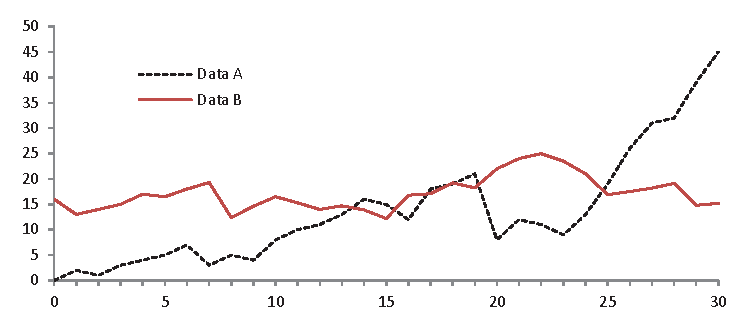
\includegraphics[width=\textwidth]{fig1.eps}
\caption{A figure caption is always placed below the illustration.
Please note that short captions are centered, while long ones are
justified by the macro package automatically.} \label{fig1}
\end{figure}

\begin{theorem}
This is a sample theorem. The run-in heading is set in bold, while
the following text appears in italics. Definitions, lemmas,
propositions, and corollaries are styled the same way.
\end{theorem}
%
% the environments 'definition', 'lemma', 'proposition', 'corollary',
% 'remark', and 'example' are defined in the LLNCS documentclass as well.
%
\begin{proof}
Proofs, examples, and remarks have the initial word in italics,
while the following text appears in normal font.
\end{proof}
For citations of references, we prefer the use of square brackets
and consecutive numbers. Citations using labels or the author/year
convention are also acceptable. The following bibliography provides
a sample reference list with entries for journal
% articles~\cite{ref_article1}, an LNCS chapter~\cite{ref_lncs1}, a
% book~\cite{ref_book1}, proceedings without editors~\cite{ref_proc1},
% and a homepage~\cite{ref_url1}. Multiple citations are grouped
% \cite{ref_article1,ref_lncs1,ref_book1},
% \cite{ref_article1,ref_book1,ref_proc1,ref_url1}.
% %
% ---- Bibliography ----
%
% BibTeX users should specify bibliography style 'splncs04'.
% References will then be sorted and formatted in the correct style.
%
\bibliographystyle{splncs04}
\bibliography{samplepaper}
% include references even if they are not cited in the text
\nocite{*}

% \begin{thebibliography}{8}
% \bibitem{ref_article1}
% Author, F.: Article title. Journal \textbf{2}(5), 99--110 (2016)

% \bibitem{ref_lncs1}
% Author, F., Author, S.: Title of a proceedings paper. In: Editor,
% F., Editor, S. (eds.) CONFERENCE 2016, LNCS, vol. 9999, pp. 1--13.
% Springer, Heidelberg (2016). \doi{10.10007/1234567890}

% \bibitem{ref_book1}
% Author, F., Author, S., Author, T.: Book title. 2nd edn. Publisher,
% Location (1999)

% \bibitem{ref_proc1}
% Author, A.-B.: Contribution title. In: 9th International Proceedings
% on Proceedings, pp. 1--2. Publisher, Location (2010)

% \bibitem{ref_url1}
% LNCS Homepage, \url{http://www.springer.com/lncs}. Last accessed 4
% Oct 2017
% \end{thebibliography}
\end{document}
